\section{XML Schema}

\begin{frame}[fragile]{CH4 XML Schema}
\begin{figure}
    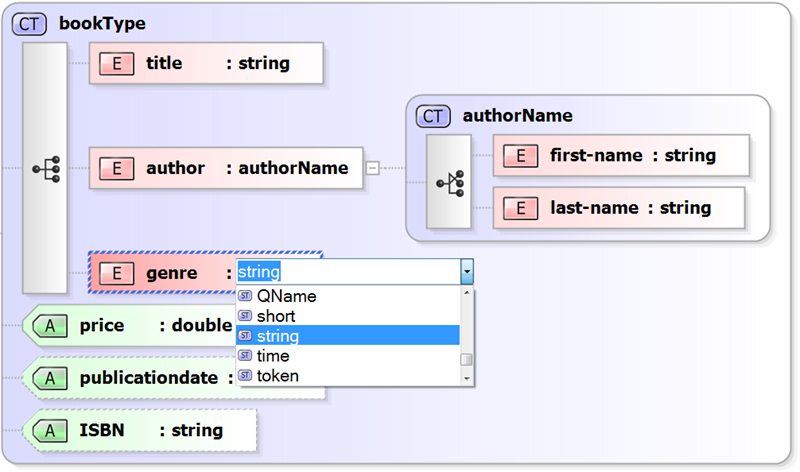
\includegraphics[width=0.9\textwidth]{figure/schema.png}
\end{figure}
\end{frame}

\begin{frame}[fragile]{本章学习目标}
\begin{easylist} \easyitem
& 理解XML Schema的含义及用途
& 掌握XML Schema的元素、属性的作用及使用方式
& 掌握XML Schema的数据类型
& 理解XML Schema的命名空间的概念
\end{easylist}
\end{frame}

\begin{frame}[fragile]{目录}
\begin{easylist} \easyitem
& XML Schema概述
& 快速入门
& 元素声明
& 属性声明
& 数据类型
&& 简单数据类型:SimpleType
&& 复杂数据类型:ComplexType
& XML Schema与命名空间
&& targetNamespace
&& elementFormDefault 与 attributeFormDefault
&& form
& 注释与注解
\end{easylist}
\end{frame}


\subsection{4.1 XML Schema概述}

\begin{frame}[fragile]{4.1 XML Schema概述}
\begin{easylist} \easyitem
& DTD本身存在的不足
&& 具有自己独特的语法,需要特定的解析技术
&& 没有数据类型的概念
&& 不支持命名空间
&& 扩展机制复杂且较为脆弱
& XML Schema是DTD的替代
&& DTD较为简单,二者会长期并存
\end{easylist}
\end{frame}


\subsection{4.2 XML Schema快速入门}

\begin{frame}[fragile]{4.2 XML Schema快速入门}
\begin{shaded}
一个Schema文档由元素、属性、命名空间和XML文档中的其他结点组成,并且至少要包含Schema根元素和XML Schema命名空间定义。
\end{shaded}
\end{frame}


\subsubsection{4.2.1 快速实例}
\begin{frame}[fragile, allowframebreaks]{4.2.1 实例—XML文档}
\begin{lstlisting}[tabsize=8, basicstyle=\small\tt, language=XML]
<?xml version="1.0"?>
<book isbn="7535421016" xmlns:xsi="http://www.w3.org/2001/XMLSchema-instance" 
       xsi:noNamespaceSchemaLocation="4-1.xsd">
    <name>康熙大帝</name>
    <author>二月河</author>
    <price>86</price>
    <pages>2012</pages>    
    <introduction>清顺治十八年,恶疾天花袭击了皇宫,皇帝爱妃
命丧黄泉,顺治痛不欲生,立意遁入空门。危急之际...</introduction>
    <publish>
        <publisher>长江文艺出版社</publisher>
        <pubDate>2006-01-01</pubDate>
    </publish>    
</book>
\end{lstlisting}
\begin{easylist} \easyitem
& 行2中的“xmlns:xsi”属性表示命名空间xsi(XML Schema Instance)为一个XML Schema实例
& 通过xsi:noNamespaceSchemaLocation与指定的XML Schema文件4-1.xsd建立关联,实现有效性验证
\end{easylist}
\end{frame}

\begin{frame}[fragile, allowframebreaks]{实例—Schema文档}
\begin{lstlisting}[tabsize=8, basicstyle=\small\tt, language=XML]
<?xml version="1.0" encoding="UTF-8"?>
<xsd:schema xmlns:xsd="http://www.w3.org/2001/XMLSchema">
    <xsd:element name="book">
        <xsd:complexType>
            <xsd:sequence>
                <xsd:element name="name" type="xsd:string"/>
                <xsd:element name="author" type="xsd:string"/>
                <xsd:element name="price" type="xsd:integer"/>
                <xsd:element name="pages" type="xsd:integer"/>
                <xsd:element name="introduction" type="xsd:string"/>
                <xsd:element name="publish" minOccurs="0" maxOccurs="1">
                    <xsd:complexType>
                        <xsd:sequence>
                            <xsd:element name="publisher" type="xsd:string"/>
                            <xsd:element name="pubDate" type="xsd:date"/>
                        </xsd:sequence>
                    </xsd:complexType>
                </xsd:element>
            </xsd:sequence>
            <xsd:attribute name="isbn" type="xsd:string"/>
        </xsd:complexType>
    </xsd:element>
</xsd:schema>
\end{lstlisting}

\begin{easylist} \easyitem
& 每一个XML Schema文档都以schema作为根元素,并位于命名空间“http://www.w3.org/2001/XMLSchema”之中
& 推荐使用的命名空间前缀有两种常见方式
&&  xsd:XML Schema Document的缩写表示
&& xs:XML Schema的缩写表示
\end{easylist}
\end{frame}


\subsubsection{4.2.2 Schema文档结构}
\begin{frame}[fragile]{4.2.2 Schema文档结构}
\begin{easylist} \easyitem
& Schema文档构成
&& 定义命名空间
&& 定义根元素的名字和类型
&& 定义子元素的名字和类型,并说明和根元素的关系
& 简单Schema文档
\begin{lstlisting}[tabsize=8, basicstyle=\small\tt, language=XML]
<?xml version="1.0" encoding="UTF-8"?>
<xsd:schema xmlns:xsd="http://www.w3.org/2001/XMLSchema">
    <!-- 详细声明内容 -->
</xsd:schema>
\end{lstlisting}
\end{easylist}
\end{frame}


\begin{frame}[fragile]{Schema文档可以树状方式查看}
\begin{figure}
    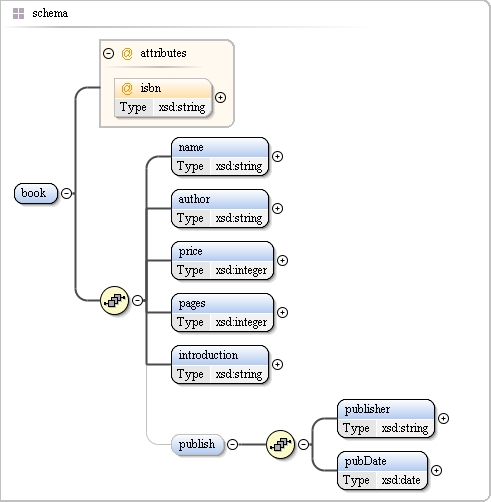
\includegraphics[width=0.75\textwidth]{figure/schema-tree.png}
\end{figure}
\end{frame}


\subsubsection{4.2.3 引用方式}
\begin{frame}[fragile]{4.2.3 引用方式}
\begin{easylist} \easyitem
& 最为常见的引用方式示例:
\begin{lstlisting}[tabsize=8, basicstyle=\small\tt, language=XML]
<book isbn="7535421016" xmlns:xsi="http://www.w3.org/2001/XMLSchema-instance" 
    xsi:noNamespaceSchemaLocation="4-1.xsd">
    <!-- XML文档内容…… -->
</book>
\end{lstlisting}
\end{easylist}
\end{frame}


\subsubsection{4.2.4 包含与导入}
\begin{frame}[fragile]{4.2.4 包含与导入}
\begin{easylist} \easyitem
& 借助于包含(include)或导入(import)机制,一个主模式文档可以由多个模式文档组合而成
&& 当其他模式文档与主模式文档具有相同的目标命名空间时,可以使用包含方式
&& 当各自拥有不同的目标命名空间时,则使用导入方式
& 适用于复杂场景
\end{easylist}
\end{frame}



\subsection{4.3 XML Schema的元素声明}

\begin{frame}[fragile]{4.3 XML Schema的元素声明}
\begin{shaded}
XML Schema通过element语法对元素进行声明,支持元素的类型名称、数据类型以及默认值、固定值等设置,元素可以是简单类型,也可以是复杂类型
\end{shaded}
\end{frame}


\subsubsection{4.3.1 schema根元素}
\begin{frame}[fragile]{4.3.1 schema根元素}
\begin{easylist} \easyitem
&  Schema文档都必须定义一个名称为schema的根元素
&& 该元素包含8个可选的属性,分别为attributeFormDefault、blockDefault、elementFormDefault、finalDefault、id、targetNamespace、version、xml:lang
& 简单示例
\begin{lstlisting}[tabsize=8, basicstyle=\small\tt, language=XML]
<?xml version="1.0" encoding="UTF-8"?>
<xsd:schema id="mySchema" xmlns:xsd="http://www.w3.org/2001/XMLSchema">
    <!-- XML Schema文档的详细定义 -->
</xsd:schema>
\end{lstlisting}
&& 可选的id属性为了方便用户的使用
&& 对应的名称空间为: http://www.w3.org/2001/XMLSchema
\end{easylist}
\end{frame}


\subsubsection{4.3.2 element元素}
\begin{frame}[fragile]{4.3.2 element元素}
\begin{easylist} \easyitem
&  element元素用于声明元素的属性,语法如下:
\begin{lstlisting}[tabsize=8, basicstyle=\small\tt, language=XML, numbers=none]
<xsd:element name="元素名称" type="元素类型"/>
\end{lstlisting}
&& name是元素类型的名称
&& 必选的type属性用于说明元素的数据类型

&  例子
\begin{lstlisting}[tabsize=8, basicstyle=\small\tt, language=XML, numbers=none]
<xsd:element name="title" type="xsd:string"/>
\end{lstlisting}
\end{easylist}
\end{frame}


\subsubsection{4.3.3 elment元素的默认值和固定值}
\begin{frame}[fragile]{4.3.3 elment元素的默认值和固定值}
\begin{easylist} \easyitem
& default属性
\begin{lstlisting}[tabsize=8, basicstyle=\small\tt, language=XML, numbers=none]
<xsd:element name="gender" type="xsd:string" default="男"/>
\end{lstlisting}
&& 当对应元素为空时,填入默认值
&& “空”的定义与数据类型相关
&&& 例如string,本身就允许空值,因此其默认值不会被填充
&&& integer数据类型的空元素会被认为是空的,并将填入默认值
&&& 如果元素的xsi:nil属性被设置为true,也不会插入默认值

& fixed属性
&& 元素值不能被改写,必须与fixed中所指定的值保持等价
&& 等价并不意味形式完全一样
\end{easylist}
\end{frame}


\begin{frame}[fragile]{元素默认值行为举例}
\begin{easylist} \easyitem
& Schema文档
\begin{lstlisting}[tabsize=8, basicstyle=\small\tt, language=XML]
<?xml version="1.0" encoding="UTF-8"?>
<xsd:schema xmlns:xsd="http://www.w3.org/2001/XMLSchema">
    <xsd:element name="name" type="xsd:string"/>
    <xsd:element name="author" type="xsd:string" default="佚名"/>
    <xsd:element name="price" type="xsd:integer" default="20"/>
</xsd:schema>
\end{lstlisting}
\end{easylist}
\end{frame}


\begin{frame}[fragile]{元素默认值行为举例}
\begin{easylist} \easyitem
& 指定值: 前后不变
&& 扩充前: <author>霍金</author>
&& 扩充后: <author>霍金</author>

& 空元素(string): 字符串的默认值不填充
&& 扩充前: <author></author>
&& 扩充后: <author></author>

& 空元素(integer): 整数类型的默认值自动填充
&& 扩充前: <price></price>
&& 扩充后: <price>20</price>

& 元素为空: 保持不变
&& 扩充前: <price xsi:nil="true"/>
&& 扩充后: <price xsi:nil="true"/>
\end{easylist}
\end{frame}



\begin{frame}[fragile]{元素固定值行为举例}
\begin{easylist} \easyitem
& Schema文档
\begin{lstlisting}[tabsize=8, basicstyle=\small\tt, language=XML, numbers=none]
<xsd:element name="count" type="xsd:integer" fixed="10"/>
\end{lstlisting}
& 有效实例
\begin{lstlisting}[tabsize=8, basicstyle=\small\tt, language=XML]
    <count>10</count>
    <count>010</count>
    <count>+10</count>
    <count></count>
    <count/>
\end{lstlisting}
\end{easylist}
\end{frame}



\subsubsection{4.3.4 元素的引用和替代}
\begin{frame}[fragile]{4.3.4 元素的引用和替代}
\begin{easylist} \easyitem
& 目的
&& 通过全局元素声明和元素引用,利用ref属性与已定义的元素进行关联
&& 避免重复定义
&& 如下例中的第20行和27行
\end{easylist}
\end{frame}


\begin{frame}[fragile, allowframebreaks]{示例文档}
\begin{lstlisting}[tabsize=8, basicstyle=\small\tt, language=XML]
<?xml version="1.0" encoding="UTF-8"?>
<xsd:schema xmlns:xsd="http://www.w3.org/2001/XMLSchema">
    <xsd:element name="book">
        <xsd:complexType>
            <xsd:sequence>
                <xsd:element name="name" type="xsd:string"/>
                <xsd:element name="author" type="xsd:string"/>
                <xsd:element name="price" type="xsd:decimal"/>
                <xsd:element name="introduction" type="xsd:string"/>
            </xsd:sequence>
        </xsd:complexType>
    </xsd:element>
    
    <xsd:element name="books">
        <xsd:complexType>
            <xsd:sequence>
                <xsd:element name="computer-books">
                    <xsd:complexType>
                        <xsd:sequence>
                            <xsd:element ref="book" maxOccurs="10"/>
                        </xsd:sequence>
                    </xsd:complexType>
                </xsd:element>
                <xsd:element name="math-books">
                    <xsd:complexType>
                        <xsd:sequence>
                            <xsd:element ref="book" maxOccurs="10"/>
                        </xsd:sequence>
                    </xsd:complexType>
                </xsd:element>
            </xsd:sequence>
        </xsd:complexType>
    </xsd:element>
</xsd:schema>
\end{lstlisting}
\end{frame}



\subsection{4.4 XML Schema的属性声明}

\begin{frame}[fragile]{4.4 XML Schema的属性声明}
\begin{easylist} \easyitem
& 通过attribute元素进行属性声明
& 属性声明与元素声明的区别
&& 属性的类型只能是简单类型
&& 属性不能包含子属性,而元素可以包含子元素
&& 属性之间没有顺序要求
\end{easylist}
\end{frame}


\subsubsection{4.4.1 属性声明}
\begin{frame}[fragile]{4.4.1 属性声明}
\begin{easylist} \easyitem
&  语法形式:
\begin{lstlisting}[tabsize=8, basicstyle=\small\tt, language=XML, numbers=none]
<xsd:attribute name="属性名称" type="属性类型"/>
\end{lstlisting}
& Example:
\begin{lstlisting}[tabsize=8, basicstyle=\small\tt, language=XML, numbers=none]
<xsd:attribute name="类别" type="xsd:string"/>
\end{lstlisting}
& 支持全局属性声明和属性引用,以提高复用程度
\end{easylist}
\end{frame}


\begin{frame}[fragile]{use属性}
\begin{easylist} \easyitem
&  use属性用于指示所声明的属性是否在XML文档中必须出现
& 取值:
&& optional:
&&& 可选属性,所声明的属性可以出现,也可以不出现,为use属性的默认值。
&& required
&&& 该属性必须指定,不能缺省。
&& prohibited
&&& 禁止在元素上使用该属性,等同于把该属性删除掉。
\end{easylist}
\end{frame}


\begin{frame}[fragile]{例子}
\begin{lstlisting}[tabsize=8, basicstyle=\small\tt, language=XML]
<?xml version="1.0" encoding="UTF-8"?>
<xsd:schema xmlns:xsd="http://www.w3.org/2001/XMLSchema">
    <xsd:attribute name="code" type="xsd:string"/>
    
    <xsd:element name="course">
        <xsd:complexType>
            <xsd:sequence>
                <xsd:element name="title" type="xsd:string"/>
                <xsd:element name="teacher" type="xsd:string"/>
            </xsd:sequence>
            <xsd:attribute ref="code" use="required"/>
            <xsd:attribute name="location" type="xsd:string" use="prohibited"/>
        </xsd:complexType>
    </xsd:element>
</xsd:schema>
\end{lstlisting}
\end{frame}


\subsubsection{4.4.2 指派属性类型}
\begin{frame}[fragile]{4.4.2 指派属性类型}
\begin{easylist} \easyitem
&  属性不能包含子元素和属性,一定是简单类型,指定方式:
&& 在属性声明中通过type属性指定为简单类型
&& 通过simpleType以匿名类型的方式为属性指定类型
&& 不明确指定属性的类型,
&&& 此时属性的类型为anySimpleType,可以是任意合法的属性取值
\end{easylist}
\end{frame}


\begin{frame}[fragile, allowframebreaks]{例子}
\begin{lstlisting}[tabsize=8, basicstyle=\small\tt, language=XML]
<?xml version="1.0" encoding="UTF-8"?>
<xsd:schema xmlns:xsd="http://www.w3.org/2001/XMLSchema">
    <xsd:attribute name="code" type="xsd:string"/>
    <xsd:attribute name="classroom"/>
    <xsd:attribute name="category">
        <xsd:simpleType>
            <xsd:restriction base="xsd:string">
                <xsd:enumeration value="专业选修"/>
                <xsd:enumeration value="专业必修"/>
            </xsd:restriction>
        </xsd:simpleType>
    </xsd:attribute>
</xsd:schema>
\end{lstlisting}
\begin{easylist} \easyitem
& 行4~11以simpleType匿名方式声明category属性
& 行12的classroom的属性类型取默认值anySimpleType
\end{easylist}
\end{frame}


\subsubsection{4.4.3 属性的默认值和固定值}
\begin{frame}[fragile]{4.4.3 属性的默认值和固定值}
\begin{easylist} \easyitem
& 默认值和固定值分别通过default和fixed属性进行设置
&& 二者不能同时出现,定义和扩充的方式与element元素中的方式一致
&& 指定了默认值的属性在XML实例中没有出现,则该属性及其默认值会被填入
&& 指定了固定值的属性,如果在XML实例中出现,所指定的属性值应和Schema中定义的固定值相等,如未指定,则该属性及其固定值会被自动填入
\end{easylist}
\end{frame}


\begin{frame}[fragile, allowframebreaks]{例子}
\begin{lstlisting}[tabsize=8, basicstyle=\small\tt, language=XML]
<?xml version="1.0" encoding="UTF-8"?>
<xsd:schema xmlns:xsd="http://www.w3.org/2001/XMLSchema">
    <xsd:element name="course">
        <xsd:complexType>
            <xsd:sequence>
                <xsd:element name="title" type="xsd:string"/>
            </xsd:sequence>
            <xsd:attribute name="periods" type="xsd:integer" default="3"/>
            <xsd:attribute name="location" type="xsd:string" fixed="ROOM-403"/>
        </xsd:complexType>
    </xsd:element>
</xsd:schema>
\end{lstlisting}

\newpage
\begin{lstlisting}[tabsize=8, basicstyle=\small\tt, language=XML]
<?xml version="1.0" encoding="UTF-8"?>
<course xmlns:xsi="http://www.w3.org/2001/XMLSchema-instance" 
    xsi:noNamespaceSchemaLocation="4-7.xsd" periods="4">
    <title>XML原理与应用</title>
</course>
\end{lstlisting}
\end{frame}



\subsection{4.5 XML Schema的数据类型}
\begin{frame}[fragile]{4.5 XML Schema的数据类型}
\begin{easylist} \easyitem
& 简单类型
&& 内置的简单数据类型
&& 用户通过simpleType自定义的简单数据类型
& 复杂类型
&& 通过complexType进行定义
\end{easylist}
\end{frame}


\subsubsection{4.5.1 简单数据类型:SimpleType}
\begin{frame}[fragile]{4.5.1 简单数据类型:SimpleType}
\begin{easylist} \easyitem
& 原子类型
&& 内置数据类型
&&& 原始数据类型(Primitive)
&&& 派生数据类型(Derived)
&& 自定义简单类型
& 列表类型
& 联合类型
\end{easylist}
\end{frame}


\begin{frame}[fragile]{4.5.1.1 内置简单类型}
\begin{easylist} \easyitem
& 内置数据类型可以用来描述元素的内容和属性取值,或者组合生成其他自定义数据类型。
& 包括原始数据类型(Primitive)和派生数据类型(Derived)两类
\end{easylist}
\end{frame}


\begin{frame}[fragile]{常用的原始数据类型}
\begin{table}[!hbp] 
\begin{tabular}{|l|l|}
\Xhline{1.3pt}
类型 & 描述 \\ \Xhline{1.3pt}
string & 字符串\\ \hline
boolean & 代表真假的布尔值\\ \hline
decimal & 十进制数字\\ \hline
float & 32位单精度浮点数\\ \hline
double & 64位双精度浮点数\\ \hline
date & 阳历日期\\ \hline
time & 每天中任何一个时刻,如18:36:16\\ \hline
dateTime& 阳历日期和某一天时间组合而成的某个时刻\\ \hline
\end{tabular}
\end{table}
\end{frame}


\begin{frame}[fragile]{常用的派生数据类型}
\begin{table}[!hbp] 
\begin{tabular}{|l|l|}
\Xhline{1.3pt}
类型 & 描述 \\ \Xhline{1.3pt}
integer & 任意长度的整数类型 \\ \hline
long & 64位有符号整数 \\ \hline
int & 32位有符号整数 \\ \hline
byte & 8位有符号整数 \\ \hline
unsignedInt & 32位无符号整数 \\ \hline
negativeInteger & 任意长度的负整数类型 \\ \hline
nonNegativeInteger & 大于等于零的整数 \\ \hline
normalizedString & 将回车、换行、制表符已转为空格 \\ \hline
\end{tabular}
\end{table}
\end{frame}


\begin{frame}[fragile]{XML Schema内置数据类型的层次结构}
\begin{figure}
    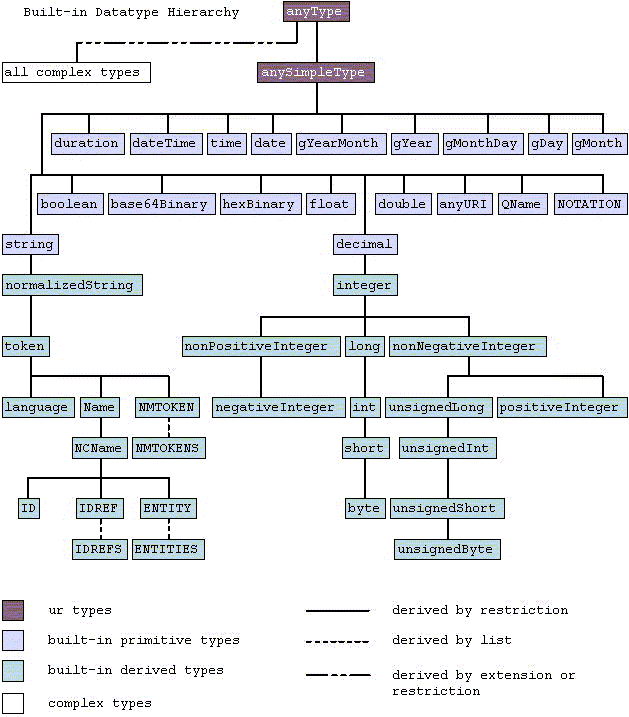
\includegraphics[width=0.75\textwidth]{figure/schema-type-hierarchy.png}
\end{figure}
\end{frame}


\begin{frame}[fragile]{4.5.1.2 自定义简单类型}
\begin{easylist} \easyitem
& 根据已经存在的简单数据类型通过simpleType关键字进行定义
& 总是通过对一个已有简单类型进行约束(restriction)派生出来
& 用户自定义的简单数据类型语法:
\begin{lstlisting}[tabsize=8, basicstyle=\small\tt, language=XML, numbers=none]
<xsd:simpleType name="自定义数据类型的名称">
    <xsd:restriction base="所基于的简单数据类型的名称">
        <!-- 约束面 -->
    </xsd:restriction>
</xsd:simpleType>
\end{lstlisting}
&& 自定义简单类型通过restriction元素对现有类型进行约束
&& 约束面
\end{easylist}
\end{frame}


\begin{frame}[fragile]{simpleType的约束面}
\begin{table}[!hbp] 
\begin{tabular}{|l|l|}
\Xhline{1.3pt}
属性 & 描述 \\ \Xhline{1.3pt}
pattern & 采用正则表达式方式限定数据的显示格式 \\ \hline
enumeration & 限定用户的取值为指定的数据集合 \\ \hline
length & 指定数据的长度 \\ \hline
maxExclusive & 指定数据的最大值(取值小于该指定值) \\ \hline
maxInclusive & 指定数据的最大值(取值小于或等于该指定值) \\ \hline
maxLength & 指定长度的最大值 \\ \hline
minExclusive & 指定数据的最小值(取值大于该指定值) \\ \hline
minInclusive & 指定数据的最小值(取值大于或等于该指定值) \\ \hline
minLength & 指定最小长度 \\ \hline
whiteSpace & 决定应用程序如何处理元素内容中的空白符 \\ \hline
totalDigits & 限定数字的最多位数 \\ \hline
fractionDigits & 限定最大的小数位,用于控制精度 \\ \hline
\end{tabular}
\end{table}
\end{frame}


\begin{frame}[fragile]{示例}
\begin{shaded}
<mobile>13800138000</ mobile >是描述一个手机号码的XML片段,此标记中的内容必须为数字,长度为固定的11位
\end{shaded}

\begin{lstlisting}[tabsize=8, basicstyle=\small\tt, language=XML]
<xsd:simpleType name="mobileType">
    <xsd:restriction base="xsd:string">
        <xsd:length value="11"/>
        <xsd:pattern value="\d{11}"/>
    </xsd:restriction>
</xsd:simpleType>
\end{lstlisting}
\end{frame}


\begin{frame}[fragile]{练习}
\begin{easylist} \easyitem
& 定义一个整数,其取值范围为[10, 100]
& 定义一个字符串,最少由4个字符组成,最多由16个字符组成
& 定义一个性别类型,其取值只能为“男”或“女”
\end{easylist}
\end{frame}


\begin{frame}[fragile]{4.5.1.3 列表类型与联合类型}
\begin{easylist} \easyitem
& 列表类型所定义的元素或属性的值可以包含多个原子值,这些并列的原子值之间通过空格分隔。列表元素使用list元素进行定义
& 语法:
\begin{lstlisting}[tabsize=8, basicstyle=\small\tt, language=XML, numbers=none]
<xsd:simpleType name="列表类型名">
    <xsd:list itemType="某一原子类型"/>
</xsd:simpleType>
\end{lstlisting}
\end{easylist}
\end{frame}


\begin{frame}[fragile]{列表类型示例}
\begin{lstlisting}[tabsize=8, basicstyle=\small\tt, language=XML]
<xsd:element name="years" type="yearListType"/>
<xsd:simpleType name="yearType">
    <xsd:restriction base="xsd:string">
        <xsd:pattern value="\d{4}"/>
    </xsd:restriction>
</xsd:simpleType>
<xsd:simpleType name="yearListType">
    <xsd:list itemType="yearType"/>
</xsd:simpleType>
\end{lstlisting}

\begin{lstlisting}[tabsize=8, basicstyle=\small\tt, language=XML, numbers=none]
<years>2010 2011 2012</years>
\end{lstlisting}
\end{frame}


\begin{frame}[fragile]{联合类型}
\begin{easylist} \easyitem
& 语法:
\begin{lstlisting}[tabsize=8, basicstyle=\small\tt, language=XML, numbers=none]
<xsd:simpleType name="联合类型名">
<xsd:union memberTypes="简单类型1 简单类型2 ……"/>
</xsd:simpleType>
\end{lstlisting}
&& 联合类型可以包含多个简单类型,所包含的简单类型既可以是原子类型,也可以是列表类型
&& 取值可以是memberTypes属性值中所指明的某一个简单类型的实例
\end{easylist}
\end{frame}


\begin{frame}[fragile]{联合类型示例}
\begin{lstlisting}[tabsize=8, basicstyle=\small\tt, language=XML]
<xsd:element name="whichYear" type="yearUnionType"/>
<xsd:simpleType name="yearUnionType">
    <xsd:union memberTypes="xsd:date yearListType"/>
</xsd:simpleType>
\end{lstlisting}

\par 正确用例:
\begin{lstlisting}[tabsize=8, basicstyle=\small\tt, language=XML]
<whichYear>2008-02-09</whichYear>
<whichYear>2010</whichYear>
\end{lstlisting}

\par 错误用例:
\begin{lstlisting}[tabsize=8, basicstyle=\small\tt, language=XML]
<whichYear>2008-02-09 2010</whichYear>
<whichYear>2010年</whichYear>
\end{lstlisting}
\end{frame}


\subsubsection{4.5.2 复杂数据类型:ComplexType}
\begin{frame}[fragile]{4.5.2 复杂数据类型:ComplexType}
\begin{easylist} \easyitem
& 四种复杂数据类型
&& 只包含文本的简单内容类型
&& 只包含子元素的纯元素内容类型
&& 包含子元素和文本的混合内容类型
&& 空元素
\end{easylist}
\end{frame}


\begin{frame}[fragile]{复杂数据类型的基本语法形式}
\begin{lstlisting}[tabsize=8, basicstyle=\small\tt, language=XML, numbers=none]
<xsd:complexType name="名称" id=ID mixed=BOOLEAN: false>
    <xsd:annotation | simpleContent | complexContent | group | all | choice | sequence | attribute | attributeGroup | anyAttribute>...
</xsd:complexType>
\end{lstlisting}
\begin{easylist} \easyitem
& name 复杂类型的名称
& id 该元素的ID,可选项
& mixed,可选布尔类型,该复杂类型的子元素之中是否允许出现字符数据,默认值为false
\end{easylist}
\end{frame}


\begin{frame}[fragile]{复杂类型的内容模型}
\begin{easylist} \easyitem
& 复杂类型的内容模型指复杂类型子元素的顺序和结构称
&& 内容模型不依赖于属性,但允许有属性
&& complexType下可以创建的内容模型有
&&& simpleContent、complexContent、sequence、group、all、choice、annotation
\end{easylist}
\end{frame}


\begin{frame}[fragile]{4.5.2.1 simpleContent}
\begin{easylist} \easyitem
& 用于从简单类型派生复杂类型
& 适用于元素包含字符内容和属性但不包含子元素的情况
& 简单内容模型的复杂类型可以包含属性,而简单类型不可
& 语法:
\begin{lstlisting}[tabsize=8, basicstyle=\small\tt, language=XML, numbers=none]
<xsd:simpleContent id=ID >
    <xsd:annotation | restriction | extension>...
</xsd:simpleContent>
\end{lstlisting}
\end{easylist}
\end{frame}


\begin{frame}[fragile, allowframebreaks]{simpleContent示例}
\begin{lstlisting}[tabsize=8, basicstyle=\small\tt, language=XML]
<?xml version="1.0" encoding="UTF-8"?>
<xsd:schema xmlns:xsd="http://www.w3.org/2001/XMLSchema">
    <xsd:element name="book">
        <xsd:complexType>
            <xsd:simpleContent>
                <xsd:extension base="xsd:string">
                    <xsd:attribute name="isbn" type="xsd:string" use="required"/>
                </xsd:extension>
            </xsd:simpleContent>
        </xsd:complexType>
    </xsd:element>
</xsd:schema>
\end{lstlisting}

\newpage
\begin{lstlisting}[tabsize=8, basicstyle=\small\tt, language=XML]
<?xml version="1.0" encoding="UTF-8"?>
<book xmlns:xsi="http://www.w3.org/2001/XMLSchema-instance"
      xsi:noNamespaceSchemaLocation="4-8.1.xsd"
      isbn="6-666-66666-6">
      XML原理与应用
</book>
\end{lstlisting}
\end{frame}


\begin{frame}[fragile]{4.5.2.2 complexContent}
\begin{easylist} \easyitem
& 用于对复杂数据类型进行扩展或限制,从复杂类型派生新的复杂类型
& 语法:
\begin{lstlisting}[tabsize=8, basicstyle=\small\tt, language=XML, numbers=none]
<xsd:complexContent id=ID mixed=true|false>
    <xsd:annotation | restriction | extension>...
</xsd:simpleContent>
\end{lstlisting}
\end{easylist}
\end{frame}


\begin{frame}[fragile, allowframebreaks]{complexContent示例}
\begin{lstlisting}[tabsize=8, basicstyle=\small\tt, language=XML]
<?xml version="1.0" encoding="UTF-8"?>
<xsd:schema xmlns:xsd="http://www.w3.org/2001/XMLSchema">
    <xsd:element name="student" type="studentType"/>

    <xsd:complexType name="personType">
        <xsd:sequence>
            <xsd:element name="name" type="xsd:string"/>
            <xsd:element name="age" type="xsd:integer"/>
        </xsd:sequence>
    </xsd:complexType>
    
    <xsd:complexType name="studentType">
        <xsd:complexContent>
            <xsd:extension base="personType">
                <xsd:sequence>
                    <xsd:element name="class" type="xsd:string"/>
                    <xsd:element name="major" type="xsd:string"/>
                </xsd:sequence>
            </xsd:extension>
        </xsd:complexContent>
    </xsd:complexType>
</xsd:schema>
\end{lstlisting}
\end{frame}


\begin{frame}[fragile]{4.5.2.3 顺序声明:sequence}
\begin{easylist} \easyitem
& 最为常用的内容模型定义方式
& 用于限定sequence内部的一组元素的出现顺序
& 带有minOccurs和maxOccurs两个属性,作用于整个顺序组合
\end{easylist}
\end{frame}


\begin{frame}[fragile, allowframebreaks]{sequence示例}
\begin{lstlisting}[tabsize=8, basicstyle=\small\tt, language=XML]
<?xml version="1.0" encoding="UTF-8"?>
<xsd:schema xmlns:xsd="http://www.w3.org/2001/XMLSchema">
    <xsd:element name="person" type="personType"/>
    <xsd:complexType name="personType">
        <xsd:sequence minOccurs="1" maxOccurs="10">
            <xsd:element name="name" type="xsd:string"/>
            <xsd:element name="age" type="xsd:integer"/>
        </xsd:sequence>
    </xsd:complexType>
</xsd:schema>
\end{lstlisting}

\newpage
\par 以下代码片段能够通过有效性验证?
\begin{lstlisting}[tabsize=8, basicstyle=\small\tt, language=XML]
<name>刘备</name>
<age>35</age>
<name>张飞</name>
<age>35</age>
\end{lstlisting}

\par 以下代码片段能够通过有效性验证?
\begin{lstlisting}[tabsize=8, basicstyle=\small\tt, language=XML]
<age>35</age>
<name>刘备</name>
\end{lstlisting}
\end{frame}


\begin{frame}[fragile]{4.5.2.4 选择声明:choice}
\begin{easylist} \easyitem
& 多选一
\end{easylist}

\begin{lstlisting}[tabsize=8, basicstyle=\small\tt, language=XML]
<?xml version="1.0" encoding="UTF-8"?>
<xsd:schema xmlns:xsd="http://www.w3.org/2001/XMLSchema">
    <xsd:complexType name="personType">
        <xsd:sequence minOccurs="1" maxOccurs="10">
            <xsd:element name="name" type="xsd:string"/>
            <xsd:element name="age" type="xsd:integer"/>
            <xsd:choice>
                <xsd:element name="wife" type="xsd:string"/>
                <xsd:element name="husband" type="xsd:string"/>
            </xsd:choice>
        </xsd:sequence>
    </xsd:complexType>
</xsd:schema>
\end{lstlisting}
\end{frame}



\begin{frame}[fragile]{4.5.2.5 分组声明:group}
\begin{easylist} \easyitem
& 使用方式
&& group声明
&&& 用于指定一个模型组的定义,定义该分组内包含的内容,并以schema元素的子元素形式出现;
&& group引用
&&& 对已经定义分组进行引用,此时group出现在复杂类型定义或其他模型组定义的内部。
\end{easylist}
\end{frame}

\begin{frame}[fragile, allowframebreaks]{group示例}
\begin{lstlisting}[tabsize=8, basicstyle=\small\tt, language=XML]
<?xml version="1.0" encoding="UTF-8"?>
<xsd:schema xmlns:xsd="http://www.w3.org/2001/XMLSchema">
    <xsd:group name="HeightAndWeightGroup">
        <xsd:sequence>
            <xsd:element name="height" type="xsd:integer"/>
            <xsd:element name="weight" type="xsd:integer"/>
        </xsd:sequence>
    </xsd:group>
    
    <xsd:complexType name="personType">
        <xsd:sequence minOccurs="1" maxOccurs="10">
            <xsd:element name="name" type="xsd:string"/>
            <xsd:element name="age" type="xsd:integer"/>
            <xsd:choice>
                <xsd:element name="wife" type="xsd:string"/>
                <xsd:element name="husband" type="xsd:string"/>
            </xsd:choice>
            <xsd:group ref="HeightAndWeightGroup"/>
        </xsd:sequence>
    </xsd:complexType>
</xsd:schema>
\end{lstlisting}
\end{frame}


\begin{frame}[fragile]{4.5.2.6 ALL声明:all}
\begin{easylist} \easyitem
& 元素可以在实例文档中以任意顺序出现
&& all元素的任何子元素声明,其minOccurs属性只能取0或1的值,maxOccurs属性只能取1值
& all示例:
\begin{lstlisting}[tabsize=8, basicstyle=\small\tt, language=XML]
<?xml version="1.0" encoding="UTF-8"?>
<xsd:schema xmlns:xsd="http://www.w3.org/2001/XMLSchema">
    <xsd:complexType name="personType">
        <xsd:all>
            <xsd:element name="name" type="xsd:string"/>
            <xsd:element name="age" type="xsd:integer"/>
        </xsd:all>
    </xsd:complexType>
</xsd:schema>
\end{lstlisting}
\end{easylist}
\end{frame}


\begin{frame}[fragile, allowframebreaks]{all示例 }
\begin{lstlisting}[tabsize=8, basicstyle=\small\tt, language=XML]
<?xml version="1.0" encoding="UTF-8"?>
<xsd:schema xmlns:xsd="http://www.w3.org/2001/XMLSchema">
    <xsd:group name="HeightAndWeightGroup">
        <xsd:sequence>
            <xsd:element name="height" type="xsd:integer"/>
            <xsd:element name="weight" type="xsd:integer"/>
        </xsd:sequence>
    </xsd:group>
    
    <xsd:complexType name="personType">
        <xsd:sequence minOccurs="1" maxOccurs="10">
            <xsd:element name="name" type="xsd:string"/>
            <xsd:element name="age" type="xsd:integer"/>
            <xsd:choice>
                <xsd:element name="wife" type="xsd:string"/>
                <xsd:element name="husband" type="xsd:string"/>
            </xsd:choice>
            <xsd:group ref="HeightAndWeightGroup"/>
        </xsd:sequence>
    </xsd:complexType>
</xsd:schema>
\end{lstlisting}
\par 该定义方式与上一定义方式的约束效果相同。
\end{frame}



\subsection{4.6 XML Schema与命名空间}
\begin{frame}[fragile]{4.6 XML Schema与命名空间}
\begin{easylist} \easyitem
& targetNamespace
& elementFormDefault
& attributeFormDefault
\end{easylist}
\end{frame}


\subsubsection{4.6.1 targetNamespace}

\begin{frame}[fragile]{4.6.1 targetNamespace}
\begin{easylist} \easyitem
& 每一个Schema文档都可有一个命名空间,称为模式文档的目标命名空间(Target Namespace)
& 每个被全局声明所定义的元素、属性、类型或分组,都与该目标命名空间有关。
& 通过targetNamespace指定所定义元素或属性所隶属的命名空间,
&& 默认情况下仅对全局声明的元素和属性起作用(未设置elementFormDefault和attributeFormDefault)
\end{easylist}
\end{frame}


\begin{frame}[fragile]{targetNamespace示例:4-14.xsd }
\begin{lstlisting}[tabsize=8, basicstyle=\small\tt, language=XML]
<?xml version="1.0" encoding="UTF-8"?>
<xsd:schema xmlns:xsd="http://www.w3.org/2001/XMLSchema"
            targetNamespace="http://www.example.org/test">
    <xsd:element name="course">
        <xsd:complexType>
            <xsd:sequence>
                <xsd:element name="name" type="xsd:string"/>
                <xsd:element name="teacher" type="xsd:string"/>
            </xsd:sequence>
            <xsd:attribute name="code" type="xsd:string" use="required"/>
        </xsd:complexType>
    </xsd:element>
</xsd:schema>
\end{lstlisting}
\end{frame}


\begin{frame}[fragile]{targetNamespace示例:4-14.xml }
\begin{lstlisting}[tabsize=8, basicstyle=\small\tt, language=XML]
<?xml version="1.0" encoding="UTF-8"?>
<test:course xmlns:test=http://www.example.org/test
      xmlns:xsi=http://www.w3.org/2001/XMLSchema-instance
      xsi:schemaLocation="http://www.example.org/test 4-14.xsd" code="106">
    <name>数据挖掘</name>
    <teacher>夏天</teacher>
</test:course>
\end{lstlisting}
\end{frame}


\subsubsection{4.6.2 elementFormDefault与attributeFormDefault}

\begin{frame}[fragile]{4.6.2 elementFormDefault与attributeFormDefault}
\begin{easylist} \easyitem
& elementFormDefault
&& unqualified(默认值)
&&& 内部元素不受目标命名空间的约束
&& qualified
&&& 内部元素也将受到目标命名空间的约束
& attributeFormDefault
&& unqualified(默认值)
&&&  内部自定义的属性不受目标命名空间的约束
&& qualified
&&& 受目标命名空间约束
\end{easylist}
\end{frame}


\subsubsection{4.6.3 form属性}

\begin{frame}[fragile]{4.6.3 form属性}
\begin{easylist} \easyitem
& 如需要对特定元素或属性设置不同于全局的配置,可以借助于element或attribute元素的form属性
& form属性的取值和作用与全局的elementFormDefault或attributeFormDefault相似,但只作用于当前声明的对象。
\end{easylist}
\end{frame}



\subsection{4.7 XML Schema的注释与注解}
\begin{frame}[fragile]{4.7 XML Schema的注释与注解}
\begin{easylist} \easyitem
& 注释:
&& 可以在模式文档中任意插入XML注释,只要符合XML的语法规定即可
& annotation
&& 增强模式文档的机器可读性
&& 不仅提供文档信息,还提供程序信息,允许模式文档使用读者可以理解和机器可以识别的信息来注释
&& 语法:
\begin{lstlisting}[tabsize=8, basicstyle=\small\tt, language=XML, numbers=none]
<xsd:annotation id=ID >
    <xsd:appinfo | documentation>...
</xsd:annotation>
\end{lstlisting}
\end{easylist}
\end{frame}


\begin{frame}[fragile, allowframebreaks]{注解应用示例 }
\begin{lstlisting}[tabsize=8, basicstyle=\small\tt, language=XML]
<?xml version="1.0" encoding="UTF-8"?>
<xsd:schema xmlns:xsd="http://www.w3.org/2001/XMLSchema">
    <xsd:element name="course" type="courseType"/>
    
    <xsd:annotation>
        <xsd:appinfo source="4-18.html"/>
        <xsd:documentation xmlns:html="http://www.w3.org/1999/xhtml">
            <html:p>注解使用示例,下面所声明的<html:strong>courseType</html:strong>自定义复杂类型,为课程类型,包含两个子元素和一个属性。</html:p>
        </xsd:documentation>
    </xsd:annotation>
    <xsd:complexType name="courseType">
        <xsd:sequence>
            <xsd:element name="name" type="xsd:string"/>
            <xsd:element name="teacher" type="xsd:string" form="unqualified"/>
        </xsd:sequence>
        <xsd:attribute name="code" type="xsd:string" form="qualified" use="required">
            <xsd:annotation>
                <xsd:documentation>必须有课程代号属性code</xsd:documentation>
            </xsd:annotation>
        </xsd:attribute>
    </xsd:complexType>
</xsd:schema>
\end{lstlisting}
\end{frame}


\begin{frame}
\begin{center}
    \Huge END
\end{center}
\begin{figure}
    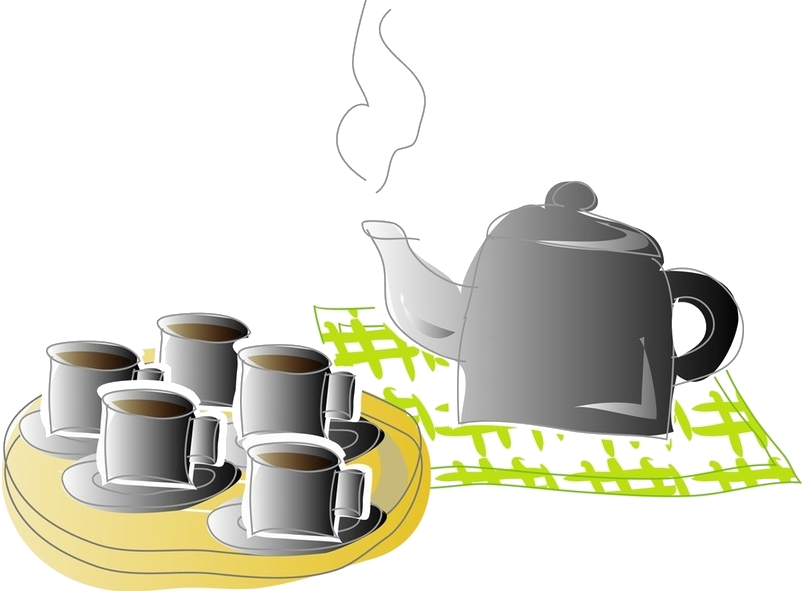
\includegraphics[width=0.75\textwidth]{figure/relax.png}
\end{figure}
\end{frame}

